\documentclass{beamer}
\usepackage[utf8]{inputenc}
\usepackage[english]{babel}
\title{Haptic terrain exploration with robotic arm}
\author{Martin Burian}
\date{\today}
\usetheme{Singapore}
\usecolortheme{default}
\usepackage{graphicx}
\usepackage{mdwlist}
\usepackage{listings}
\usepackage{comment}
\usepackage{color}
\usepackage{array}
\usepackage{algorithm}
\usepackage{algpseudocode}

\graphicspath{{.}{../figures/}}

\newcommand\mytextbullet{\leavevmode\usebeamertemplate{itemize item}}

\providecommand*{\diff}{\textrm{d}\,}
\providecommand*{\pdiff}{\partial\,}
\newcommand*{\m}[1]{\(#1\)}
\newcommand*{\unit}[1]{\; \textrm{[#1]}}
\newcommand*{\degr}{^\circ}
\newcommand*{\uvz}[1]{``#1''}
\newcommand*{\quot}[2]{\textit{\uvz{#1}}\cite{#2}}
\renewcommand*{\vec}[1]{\mathbf{#1}}
\newcommand*{\mat}[1]{\mathbf{#1}}
\newcommand*{\half}{^1\!/_{\!2}}
\newcommand*{\difrac}[2]{^{#1\!}/_{\!#2}}
\newcommand*{\R}{I\!\!R}
\newcommand*\colvec[3][]{
    \begin{pmatrix}\ifx\relax#1\relax\else#1\\\fi#2\\#3\end{pmatrix}
}
\newcommand*{\dvec}[1]{\dot{\vec{#1}}}
\renewcommand\mathfamilydefault{\rmdefault}
\newcommand*{\mns}{\(-\)}

\definecolor{ctublue}{rgb}{0, .423, .705}
% \definecolor { ctulightblue } { RGB }{  }
\setbeamercolor*{palette secondary}{use=structure,fg=white,bg=ctublue}
% \setbeamercolor*{palette secondary}{use=structure,fg=white,bg=\ctublue!75}

\begin{document}

\begin{frame}
  \titlepage
\end{frame}

\section{Task}
\subsection{test}

\begin{frame}
  \frametitle{Task motivation}

  \begin{columns}
    \begin{column}{0.5\textwidth}
      \begin{figure}[htp]
        \centering
        \includegraphics[width=\textwidth]{photo/robot_exploring.jpg}
      \end{figure}
    \end{column}
  
    \begin{column}{0.5\textwidth}
      \begin{itemize}
      \item search and rescue robot with arm
      \item external (light-based) sensors fail: dust, smoke
      \item[\(\rightarrow\)] explore environment with robotic arm
      \end{itemize}
    \end{column}
  
  \end{columns}

\end{frame}


\begin{frame}
  \frametitle{Optoforce sensor with extension}
  
  \begin{columns}[T]
    \begin{column}{0.39\textwidth}
      \begin{figure}[htp]
        \centering
        \includegraphics[width=3cm]{OMD-xsec.png}

        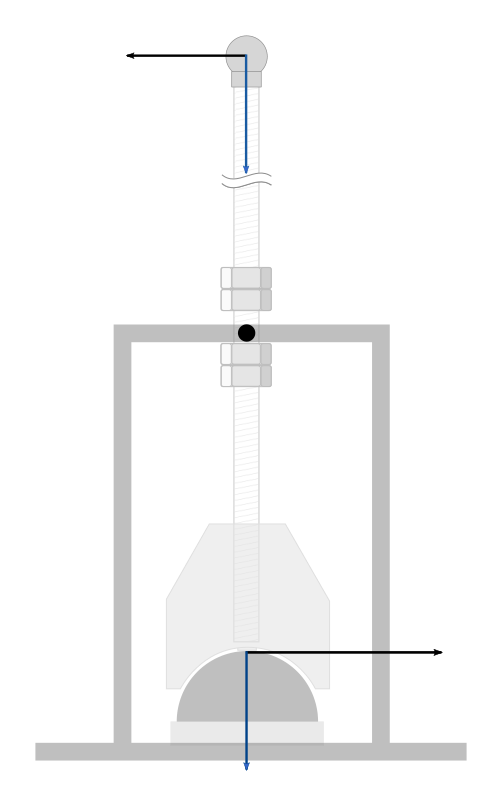
\includegraphics[width=3cm]{otpo_frame.pdf}
      \end{figure}
    \end{column}
  
    \begin{column}{0.6\textwidth}
      \vspace{-0.8cm}
      \begin{figure}[htp]
        \centering
        \includegraphics[height=9cm, angle=-30]{photo/tool.jpg}
      \end{figure}
    \end{column}
  \end{columns}
\end{frame}


\section{Mapping}
\subsection{test}


\begin{frame}
  \frametitle{Task decomposition}
  Two separate parts:

  \begin{enumerate}
  \item \textbf{generate a path} that will explore the whole environment and build the map
      \begin{itemize}
      \item map represented in dense occupancy grid
      \item formulated as a Coverage Path Planning
      \item alternatives: reinforcement learning, general planning (e.g. ILP)
      \end{itemize}

  \item \textbf{drive the robot} along the path
      \begin{itemize}
      \item motion planning (in joint space)
      \item analytical IK solution for simple linear movement (in Cartesian space)
      \end{itemize}
  \end{enumerate}
\end{frame}

\begin{frame}
  \frametitle{Algorithms for CPP}
  \begin{itemize}
    \item \textbf{exact} - decompose to trivially coverable (not usable here)
    \item geometric \textbf{neural network}
      \begin{itemize}
      \item simulate neural network, unvisited cells are externally excited
      \end{itemize}
    \item \textbf{heuristic} choice in each point, or global move
      \begin{itemize}
      \item compact space, based on knight heuristic for Hamiltonian path
      \end{itemize}

      \begin{figure}[ht]
        \centering
        \includegraphics[width=3cm]{decomp_boustrop.pdf}
        \quad
        \includegraphics[width=3cm]{expl_nn_fn.pdf}
        \includegraphics[width=3.5cm]{expl_heuristic_fn.pdf}
      \end{figure}
     \item generalization from 2D to 3D
    \end{itemize}
\end{frame}


\begin{frame}
  \frametitle{Arm control}
  To navigate the arm in Cartesian space, we can use
   \vspace{.3cm}
  \begin{itemize}
  \item \textbf{motion planning} (in joint space)
    \begin{columns}[T]
      \begin{column}{.5\textwidth}
        \begin{itemize}
        \item[+] global movement
        \item[+] libraries available
        \end{itemize}
      \end{column}
      
      \begin{column}{.5\textwidth}
        \begin{itemize}
        \item[\mns] computationally expensive
        \item[\mns] sampling-based = uncertain
        \item[\mns] not reliable around obstacles
        \end{itemize}
      \end{column}
    \end{columns}
  \item \textbf{analytical IK solution} (Jacobian pseudoinverse)
    \begin{columns}[T]
      \begin{column}{.5\textwidth}
        \begin{itemize}
        \item[+] fast computation
        \item[+] usable precision
        \end{itemize}
      \end{column}
      
      \begin{column}{.5\textwidth}
        \begin{itemize}
        \item[\mns] only simple relative movements
        \item[\mns] more difficult collision checking
        \item[\mns] handle singularities
        \end{itemize}
      \end{column}
    \end{columns}
  \end{itemize}
    \textbf{\(\rightarrow\) use both}
\end{frame}


\section{Results}
\subsection{test}

\begin{frame}
  \frametitle{Algorithm evaluation}
    \newlength{\fw}
    \setlength{\fw}{3cm}
  \begin{tabular}{rccc}
     & empty & 2D & 3D \\
    \raisebox{1.5cm}{NN} &
    \includegraphics[width=\fw]{2d_coverage_nn_empty.pdf} &
    \includegraphics[width=\fw]{2d_coverage_nn.pdf} &
    \includegraphics[width=\fw]{3d_coverage_nn.pdf} \\
    \raisebox{1.5cm}H &
    \includegraphics[width=\fw]{2d_coverage_heur_empty.pdf} &
    \includegraphics[width=\fw]{2d_coverage_heur.pdf} &
    \includegraphics[width=\fw]{3d_coverage_heur.pdf}
  \end{tabular}

\end{frame}


\begin{frame}
  \frametitle{TODO Arm control evaluation}
  \begin{columns}
    \begin{column}{.5\textwidth}
      \begin{figure}[ht]
        \centering
        Planner quirks
        \includegraphics[width=3cm]{wrong_plan_KDL.png}

        \includegraphics[width=3cm]{wrong_plan_close_obstacle.png}
      \end{figure}
    \end{column}
    \begin{column}{.5\textwidth}
      \begin{figure}[ht]
        \centering
      IK control accuracy
        \includegraphics[height=3cm]{jacob_error_real.pdf}
      \end{figure}
    \end{column}
  \end{columns}
\end{frame}


\begin{frame}
  \frametitle{TODO Experiments and conclusions}
  \begin{figure}[ht]
    \centering
    \newlength{\fww}
    \setlength{\fww}{3.4cm}
    \includegraphics[width=\fww]{photo/exp_real_stopping.jpg}
    \,
    \includegraphics[width=\fww]{photo/exp_real_empty.jpg}
    \,
    \includegraphics[width=\fww]{photo/exp_real_chair.jpg}
  \end{figure}

  \begin{itemize}
  \item the system is limited by motion planners around obstacles
  \end{itemize}
\end{frame}

\appendix

\begin{frame}
  \frametitle{}
  \centering
  \huge{Thank you}
  
\end{frame}


\begin{frame}
  \frametitle{}
\tiny{
\begin{algorithmic}
  \State \textbf{Input:}
  \State \(\vec v \gets\) Cartesian twist
  \State \(\vec p_t \gets\) target position
  \vspace{1em}

  \While{\(\vec p_t\) is not reached with tolerance \(\epsilon\)}
    \State \(\vec p \gets \) current arm state
    \Comment \parbox[t]{.4\textwidth}{Represents both joint angles and end effector position}
    \State \(\vec e_c \gets \) Cartesian error of \(\vec p\)
    
    \If{\(\vec e_c > \epsilon_{max}\)}
      \State \textbf{return} failure
    \EndIf

    \State \(\vec v_t \gets \vec v + P \vec e_c\)
    \Comment \m P is P-regulator constant

    \State \(\dvec q \gets \)computeJointVelocity(\(\vec p, \vec v_t\))
    \vspace{1em}

    \While{checkVelocityLimit(\(\dvec q\)) fails or at maximum 4 times}
      \State \(\vec v_t \gets \frac{1}{2} \vec v_t\)
      \State \(\dot{\vec q} \gets \)computeJointVelocity(\(\vec p, \vec v_t\))
    \EndWhile

    \If{checkVelocityLimit(\(\dvec q\)) fails}
      \State \textbf{return} failure
    \EndIf
    \vspace{1em}

    \State \(\vec p_n \gets \vec p + \dvec q \Delta t\)
    \Comment \parbox[t]{.4\textwidth}{\(\Delta t\) is the duration of one loop, here 20\,ms}

    \If{collisionCheck(\(\vec p_n\)) reports collision}
      \State \textbf{return} failure
    \EndIf
    \vspace{1em}

    \State publishJointVelocityTwice(\(\dvec q\))

    \State run loop at 50\,Hz
    
  \EndWhile
  \State \textbf{return} success
\end{algorithmic}}

\end{frame}


\begin{frame}
  \vspace{-0.5cm}
  \begin{figure}[ht]
    \centering
    \includegraphics[height=\textheight]{control_all.pdf}
  \end{figure}

\end{frame}



\begin{frame}
  \vspace{-0.5cm}
  \begin{figure}[ht]
    \centering
    \includegraphics[width=\textwidth]{control_jacob.pdf}
  \end{figure}

\end{frame}


\end{document}
